
\begin{frame}{Cluser Exapansion}

    \begin{minipage}{0.5\textwidth}

        \only<1-2> { 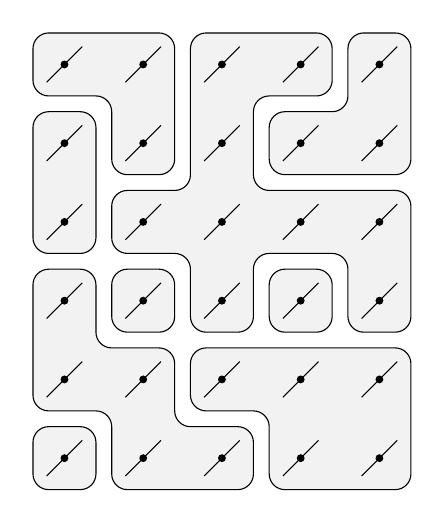
\begin{tikzpicture}[clust/.style = {rounded corners= 0.2 cm, fill=gray!10}]

                \def \e {0.40}

                \draw[clust] (1-\e,1-\e)--(1-\e,1+\e)--(1+\e,1+\e)--(1+\e,1-\e)--cycle;
                %\draw (,)--(,)--(,)--(,)--cycle;
                \draw[clust ] (3-\e,2+\e) -- (5+\e,2+\e) -- (5+\e,1-\e) -- (4-\e, 1-\e) -- (4-\e, 2-\e)-- (3-\e, 2-\e)--cycle;
                \draw[clust ] (1-\e,3+\e)--(1+\e, 3+\e)-- (1+\e,2+\e) -- (2+\e,2+\e) -- (2+\e,1+\e)--(3+\e,1+\e)-- (3+\e,1-\e)--(2-\e,1-\e)--(2-\e,2-\e) -- (1-\e,2-\e)--cycle;
                \draw[clust] (2-\e, 4-\e) -- (2-\e,4+ \e) -- (3-\e, 4+\e) -- (3-\e,6+ \e) -- (4+\e,6+ \e) -- (4+\e, 6-\e) -- (3+\e, 6-\e) -- (3+\e,4+ \e) -- (5+\e,4+ \e) -- (5+\e,3- \e) -- (5-\e,3- \e) -- (5-\e, 4-\e) -- (3+\e, 4-\e) -- (3+\e,3- \e) -- (3-\e, 3-\e)-- (3-\e, 4-\e) --cycle;
                \draw[clust] (4-\e,5-\e)--(4-\e,5+\e)--(5-\e,5+\e)--(5-\e,6+\e)--(5+\e,6+\e)--(5+\e,5-\e)--cycle;
                \draw[clust] (2-\e,3-\e)--(2-\e,3+\e)--(2+\e,3+\e)--(2+\e,3-\e)--cycle;
                \draw[clust] (4-\e,3-\e)--(4-\e,3+\e)--(4+\e,3+\e)--(4+\e,3-\e)--cycle;
                \draw[clust] (1-\e,4- \e)--(1-\e, 5+ \e)--(1+\e, 5+\e)--(1+\e, 4-\e)--cycle;
                \draw[clust] (1-\e, 6-\e)--(1-\e,6+ \e)--(2+\e, 6+ \e)--(2+\e,5- \e)--(2-\e, 5- \e)--(2-\e,6- \e)--cycle;

                \def \sz {5};

                \def \radius {0.1}
                \def \ll {0.35}

                \foreach \x in {1,2,..., 5}
                    {
                        \foreach \y in {1,2,..., 6}
                            {
                                \pgfmathtruncatemacro{\s}{\x*10+\y   }

                                \fill (\x,\y) circle (0.05cm);

                                %\node[draw=none] (O\s) at (\x,\y) {};

                                \pgfmathsetmacro{\pp}{   \x+\ll }
                                \pgfmathsetmacro{\pm}{   \x-\ll  }

                                \pgfmathsetmacro{\kp}{   \y+\ll  }
                                \pgfmathsetmacro{\km}{   \y-\ll  }

                                \node (Op\s) at (\pp,\kp) {};
                                \node (Om\s) at (\pm,\km) {};

                                \draw (\x,\y)  --  (Op\s);
                                \draw  (\x,\y) --  (Om\s);

                            }
                    }

            \end{tikzpicture}}
        \only<3>{
            \begin{itemize}
                \item Multiple choices for encoding
                \item Spurious blocks
                \item Doesn't break symmetry
                \item Thermodynamic limit
                \item Tensor Network toolbox
            \end{itemize}
        }
    \end{minipage}
    \begin{minipage}{0.49\textwidth}

        \only<1> {

            \begin{itemize}
                \item $ e^{-\beta \hat{H}} = \sum_{ \{B_i\} } \bigotimes_i B_i  $
                \item Solves local patch exactly
                \item Increase size patches
                \item Encoded by 1 tensor
                      \begin{equation}
                          \vcenter{ \hbox{ \pepob{4}{3}{{
                                              "-","-","-",
                                              "-","a","c",
                                              "-","-","-"}}{{
                                              "-","-",
                                              "-","-",
                                              "d","b",
                                              "-","-"}}{{
                                              1,1,4,1,
                                              1,4,12,4,
                                              1,1,4,1}} }}
                      \end{equation}

            \end{itemize}

        }

        \only<2-3> {
            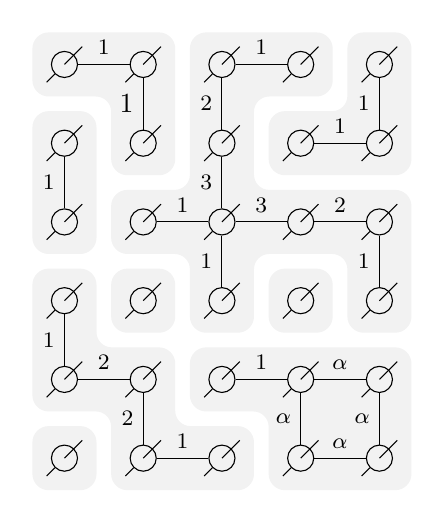
\begin{tikzpicture}[clust/.style = {rounded corners= 0.2 cm,  ,fill=gray!10, color=gray!10 }]

                \def \e {0.40}

                \draw[clust] (1-\e,1-\e)--(1-\e,1+\e)--(1+\e,1+\e)--(1+\e,1-\e)--cycle;
                %\draw (,)--(,)--(,)--(,)--cycle;
                \draw[clust ] (3-\e,2+\e) -- (5+\e,2+\e) -- (5+\e,1-\e) -- (4-\e, 1-\e) -- (4-\e, 2-\e)-- (3-\e, 2-\e)--cycle;
                \draw[clust ] (1-\e,3+\e)--(1+\e, 3+\e)-- (1+\e,2+\e) -- (2+\e,2+\e) -- (2+\e,1+\e)--(3+\e,1+\e)-- (3+\e,1-\e)--(2-\e,1-\e)--(2-\e,2-\e) -- (1-\e,2-\e)--cycle;
                \draw[clust] (2-\e, 4-\e) -- (2-\e,4+ \e) -- (3-\e, 4+\e) -- (3-\e,6+ \e) -- (4+\e,6+ \e) -- (4+\e, 6-\e) -- (3+\e, 6-\e) -- (3+\e,4+ \e) -- (5+\e,4+ \e) -- (5+\e,3- \e) -- (5-\e,3- \e) -- (5-\e, 4-\e) -- (3+\e, 4-\e) -- (3+\e,3- \e) -- (3-\e, 3-\e)-- (3-\e, 4-\e) --cycle;
                \draw[clust] (4-\e,5-\e)--(4-\e,5+\e)--(5-\e,5+\e)--(5-\e,6+\e)--(5+\e,6+\e)--(5+\e,5-\e)--cycle;
                \draw[clust] (2-\e,3-\e)--(2-\e,3+\e)--(2+\e,3+\e)--(2+\e,3-\e)--cycle;
                \draw[clust] (4-\e,3-\e)--(4-\e,3+\e)--(4+\e,3+\e)--(4+\e,3-\e)--cycle;
                \draw[clust] (1-\e,4- \e)--(1-\e, 5+ \e)--(1+\e, 5+\e)--(1+\e, 4-\e)--cycle;
                \draw[clust] (1-\e, 6-\e)--(1-\e,6+ \e)--(2+\e, 6+ \e)--(2+\e,5- \e)--(2-\e, 5- \e)--(2-\e,6- \e)--cycle;

                \def \sz {5};

                \def \radius {0.1}
                \def \ll {0.35}

                \foreach \x in {1,2,..., 5}
                    {
                        \foreach \y in {1,2,..., 6}
                            {
                                \pgfmathtruncatemacro{\s}{\x*10+\y   }

                                \node[draw, circle, radius = \radius ] (O\s) at (\x,\y) {};

                                \pgfmathsetmacro{\pp}{   \x+\ll }
                                \pgfmathsetmacro{\pm}{   \x-\ll  }

                                \pgfmathsetmacro{\kp}{   \y+\ll  }
                                \pgfmathsetmacro{\km}{   \y-\ll  }

                                \node (Op\s) at (\pp,\kp) {};
                                \node (Om\s) at (\pm,\km) {};

                                \draw (O\s.center)  --  (Op\s);
                                \draw (Om\s) --  (O\s);

                            }
                    }

                %vertical
                \draw (O12) -- node [left] {\footnotesize 1} (O13);
                \draw (O14) -- node [left] {\footnotesize 1} (O15);

                \draw (O21) -- node [left] {\footnotesize 2} (O22);
                \draw (O25) -- node [left] {1} (O26);

                \draw (O33) -- node [left] {\footnotesize 1} (O34);
                \draw (O34) -- node [left] {\footnotesize 3} (O35);
                \draw (O35) -- node [left] {\footnotesize 2} (O36);

                \draw (O41) -- node [left] {\footnotesize $\alpha$} (O42);

                \draw (O51) -- node [left] {\footnotesize $\alpha$} (O52);
                \draw (O53) -- node [left] {\footnotesize 1} (O54);
                \draw (O55) -- node [left] {\footnotesize 1} (O56);

                %horizontal

                \draw (O21) -- node [above] {\footnotesize 1} (O31);
                \draw (O41) -- node [above] {\footnotesize $\alpha$} (O51);

                \draw (O12) -- node [above] {\footnotesize 2} (O22);
                \draw (O32) -- node [above] {\footnotesize 1} (O42);
                \draw (O42) -- node [above] {\footnotesize $\alpha$} (O52);

                \draw (O24) -- node [above] {\footnotesize 1} (O34);
                \draw (O34) -- node [above] {\footnotesize 3} (O44);
                \draw (O44) -- node [above] {\footnotesize 2} (O54);

                \draw (O45) -- node [above] {\footnotesize 1} (O55);

                \draw (O16) -- node [above] {\footnotesize 1} (O26);
                \draw (O36) -- node [above] {\footnotesize 1} (O46);

            \end{tikzpicture}
        }

    \end{minipage}
\end{frame}

% \begin{frame}{Notation}
%     \begin{equation}
%         O^{0 0} = \mpo{1}{ {0,0}  }{ {"$i$",}  }{ {"$j$",}}{}{{"",}} = \mpob{1}{ {0,0}  }{ {"$i$",}  }{ {"$j$",}}{}{{"",}}
%     \end{equation}

%     \begin{equation}
%         O^{0 1} O^{1 0} = \mpob{2}{ {0,1,0}  }{ {"$i_1$","$i_2$"}  }{ {"$j_1$","$j_1$",}}{}{{"",}}
%     \end{equation}

% \end{frame}

% \begin{frame}{General idea}
%     \begin{equation}
%         \mpob{1}{ {0,0}  }{}{}{}{{"",}} = \exp \left( -\beta H(\mpob{1}{}{}{}{}{{"",}})   \right)
%     \end{equation}

%     \begin{equation}
%         \begin{split}
%             \mpob{2}{ {0,1,0}  }{}{}{}{{"",}}  = \exp -\beta H( & \mpob{2}{ {,,} }{}{}{}{{"",}}) \\
%             - &\mpob{2}{ {0,0,0}  }{}{}{}{{"",}}
%         \end{split}
%     \end{equation}

% \end{frame}

% \begin{frame}{General idea}
%     \begin{equation}
%         \begin{split}
%             \only<1> { \mpob{3}{ {0,1,1,0}  }{}{}{}{{,,,}}  = \exp -\beta H( &   \mpob{3}{ {,,,} }{}{}{}{{,,}})  \\
%                 - \; &\mpob{3}{ {0,0,0,0}  }{}{}{}{{,,,}}\\
%                 - \;&\mpob{3}{ {0,1,0,0}  }{}{}{}{{,,,}}\\
%                 - \; &\mpob{3}{ {0,0,1,0}  }{}{}{}{{,,,}}}
%             \only<2> {  \mpob{3}{ {0,1,1,0}  }{}{}{}{{,,,}}    = \exp -\beta H( &   \mpob{3}{ {,,,} }{}{}{}{{,,}})  \\[10pt]
%                 - \; &\mpob{3}{ {,,,}  }{}{}{}{{,,,}}}
%             \only<3> {  \boxed{ \mpob{3}{ {0,1,1,0}  }{}{}{}{{,,,}} } }
%         \end{split}
%     \end{equation}
% \end{frame}

% \subsection{1D}
% \begin{frame}{1D: Variant A}
%     \begin{subequations}
%         \begin{align}
%              & \mpob{1}{ {,}  }{}{}{}{{,,}}                                      \\
%              & \mpob{2}{ {,"1",}  }{}{}{}{{,,}}                                  \\
%              & \mpob{3}{ {,"1","1",}  }{}{}{}{{,,,}}                             \\
%              & \mpob{4}{ {,"1","2","1",}  }{}{}{}{{,,,,,}}    \label{2sitepatch} \\
%              & \mpob{5}{ {,"1","2","2","1",}  }{}{}{}{{,,,,,}} \; .
%         \end{align}
%     \end{subequations}
% \end{frame}

% \begin{frame}{1D: Variant E}
%     \begin{subequations}
%         \begin{align}
%              & \mpob{1}{ {,}  }{}{}{}{{,,}}                          \\
%              & \mpob{2}{ {,"1",}  }{}{}{}{{,,}}                      \\
%              & \mpob{3}{ {,"1","1'",}  }{}{}{}{{,,,}}                \\
%              & \mpob{4}{ {,"1","2","1'",}  }{}{}{}{{,,,,,}}          \\
%              & \mpob{5}{ {,"1","2","2'","1'",}  }{}{}{}{{,,,,,}} \;.
%         \end{align}
%     \end{subequations}
% \end{frame}

% \begin{frame}{1D: Variant F}
%     \begin{subequations}
%         \begin{align}
%              & \mpob{1}{ {,}  }{}{}{}{{,,}}                                         \\
%              & \mpob{2}{ {,"1'",}  }{}{}{}{{,,}}+  \mpob{2}{ {,"1",}  }{}{}{}{{,,}} \\
%              & \mpob{3}{ {,"1","1",}  }{}{}{}{{,,,}}                                \\
%              & \mpob{4}{ {,"1","2","1",}  }{}{}{}{{,,,,,}} \; +  \nonumber          \\
%              & \mpob{4}{ {,"1","2'","1",}  }{}{}{}{{,,,,,}}                         \\
%              & \mpob{5}{ {,"1","2","2","1",}  }{}{}{}{{,,,,,}} \;.
%         \end{align}
%     \end{subequations}
% \end{frame}

% \subsection{2D}

% \begin{frame}
%     \begin{equation}
%         O^{0000} =  \vcenter{ \hbox{ \pepob{4}{3}{{
%                             "-","-","-",
%                             "-","0","0",
%                             "-","-","-"}}{{
%                             "-","-",
%                             "-","-",
%                             "0","0",
%                             "-","-"}}{{
%                             1,1,4,1,
%                             1,4,12,4,
%                             1,1,4,1}} }} = \mpob{1}{ {,}  }{}{}{}{{,,}}
%     \end{equation}
% \end{frame}

% \begin{frame}{2D: Linear Blocks}
%     \begin{subequations}
%         \begin{align}
%              & \vcenter{\hbox{ \pepob{2}{2}{{"1",,}}{{,,}}{{0,0,1,1}} }}                                                                                                                                   \\[0.5cm]
%              & \vcenter{\hbox{  \pepob{2}{2}{{"1","1",}}{{"1","1",}}{{0,0,0,1}} }}\;
%             \vcenter{\hbox{  \pepob{3}{2}{{"1","1","1","1"}}{{"1","1","1","1"}}{{0,0,0,1,1,1}} }}                                                                                                          \\[0.5cm]
%              & \vcenter{\hbox{  \pepob{3}{2}{{"1","1","1","1"}}{{"1","1","1","1"}}{{0,0,0,1,0,1}} \quad   \pepob{3}{3}{{"1","1","1","1","1","1",}}{{"1","1","1","1","1","1",}}{{1,0,1,0,0,0,1,0,1}}  }} \;
%         \end{align}
%     \end{subequations}
% \end{frame}

% \begin{frame}{2D: Nonlinear Blocks}
%     \begin{equation}
%         \vcenter{\hbox{   {\pepob{2}{2}{{"$\alpha$","$\alpha$",}}{{"$\alpha$","$\alpha$",}}{{0,0,0,0}}} }}
%     \end{equation}

%     \begin{equation}
%         \vcenter{\hbox{     \pepob{5}{3}{{
%                             "-","-", "-",     "-",
%                             "-","1","$\beta$","-",
%                             "-","-","$\alpha$","-"}}{{
%                             "-","-",
%                             "-","-",
%                             "-","$\gamma$",
%                             "-","$\alpha$",
%                             "-","-"}}{{
%                             1,1,1,1,1,
%                             1,0,0,0,1,
%                             1,1,0,0,1}} }} \; .
%     \end{equation}
% \end{frame}
